\documentclass[14pt, oneside]{altsu-report}

\worktype{Отчёт по научно-исследовательской работе:}
\title{Тестер ведомых SPI устройств}
\author{Д.\,С.~Вебер}
\groupnumber{506}
\GradebookNumber{1337}
\supervisor{П.\,Н.~Уланов}
\supervisordegree{ст. пр. каф. ВТиЭ}
\ministry{Министерство науки и высшего образования}
\country{Российской Федерации}
\fulluniversityname{ФГБОУ ВО Алтайский государственный университет}
\institute{Институт цифровых технологий, электроники и физики}
\department{Кафедра вычислительной техники и электроники}
\departmentchief{В.\,В.~Пашнев}
\departmentchiefdegree{к.ф.-м.н., доцент}
\shortdepartment{ВТиЭ}
\abstractRU{	
	В ходе выполнения научно-исследовательской работы был исследован принцип работы интерфейса SPI, проведено знакомство с библиотеками для микроконтроллеров AVR и создан макет ведущего устройства. 
  
  	Цель работы --- создать макет тестера ведомых устройств, работающих по SPI интерфейсу.
  
 	 В результате выполнения научно-исследовательской работы был создан макет управляющего устройства, с помощью которого подаются различные команды ведомому устройству, работающему по SPI интерфейсу передачи данных. 
 	 }
%\abstractEN{Большой текст на английском!}
\keysRU{интерфейсы передачи данных, программирование микроконтроллеров}
\keysEN{computer simulation, distributed version control}

\date{\the\year}


% Подключение файлов с библиотекой.
\addbibresource{graduate-students.bib}
\usepackage{minted}
\usepackage{tocloft}
\renewcommand\cftchapfont{\mdseries}
\renewcommand\cftchappagefont{\mdseries}


\begin{document}
\maketitle
\setcounter{page}{2}
\makeabstract
\tableofcontents

\chapter*{Введение}
\addcontentsline{toc}{chapter}{Введение}
	На сегодняшний день разрабатывается достаточно много ведомых устройств, работающих по определённым интерфейсам передачи данных. Создание каждого из них занимает время как на проектирование, так и на отладку работы.
	
	Логично возникает вопрос с помощью чего устройства управляются и отлаживаются. Для такой задачи требуются ведущие устройства, которые передают данные ведомым. Поэтому разработка управляющих устройств несомненно остаётся необходимой и актуальной.
	
	В данной научно-исследовательской работе объектом исследования являются интерфейсы передачи данных, программирование микроконтроллеров. 
	
	Целью работы является создать рабочий макет тестера.
	
	Задачи научно-исследовательской работы:  
	\begin{enumerate}
		\item Выбрать инструменты для разработки программы.
		\item Разработать программу.
		\item Собрать макет.
		\item Проверить работоспособность.
	\end{enumerate}

\chapter{Коротко о SPI} 

	SPI (англ. Serial Peripheral Interface, SPI bus — последовательный периферийный интерфейс, шина SPI) — последовательный синхронный стандарт передачи данных в режиме полного дуплекса, предназначенный для обеспечения простого и недорогого высокоскоростного сопряжения микроконтроллеров и периферии \cite{spi}. Устройства, которые работают по протоколу SPI, используются в широком спектре областей, включая электронику, автомобильную промышленность, медицинское оборудование, промышленные системы и другие. Он может использоваться для передачи различных типов данных, таких как цифровые данные, команды, адреса и т.д. В зависимости от конкретной системы, которая использует протокол SPI, можно передавать следующие типы данных:
	\begin{enumerate}
		\item Цифровые данные: это наиболее распространенный тип данных, который передается по протоколу SPI. Это могут быть любые двоичные данные, например, изображения, звуковые файлы, видеофайлы, текстовые файлы и т.д.
		\item Команды: некоторые периферийные устройства могут требовать отправки команд для выполнения определенных задач. Команды могут содержать информацию о том, какое действие необходимо выполнить или какой регистр необходимо изменить.
		\item Адреса: если периферийное устройство имеет встроенную память, то адреса могут использоваться для чтения или записи данных в эту память.
		\item Управляющие сигналы: помимо данных и адресов, протокол SPI может использоваться для передачи различных управляющих сигналов, таких как сигналы часов, выборки устройств, и т.д.
	\end{enumerate}	 
	
	В целом, протокол SPI является очень гибким и может быть использован для передачи различных типов данных в зависимости от конкретной системы, которая использует этот протокол и существует множество устройств, которые могут работать в качестве SPI Master. Микроконтроллеры, такие как Arduino, Raspberry Pi или STM32, имеют встроенные контроллеры SPI, которые могут быть использованы в качестве мастера. Также на рынке существуют специальные микросхемы, например MAX3100 \cite{max3100}, которые могут быть использованы для работы в качестве SPI Master. В нашем случае устройство на базе Arduino будет передавать команды, благодаря которым можно будет выяснить, что ведомое устройство работает и выполняет поставленные требования.	

\chapter{Создание макета устройства} 
	Для реализации проекта была выбрана ввиду своих удобств плата на базе микроконтроллера ATmega328 --- Arduino UNO со следующими характеристиками\cite{uno}: 
	\begin{itemize}
		\item Напряжение питания: 5 В.
		\item Цифровой входы/выходы: 14 линий.
		\item Аналоговые входы: 6.
		\item Flash-память: 32 кб.
		\item Оперативная память: 2 кб.
		\item Встроенные интерфейсы: i2c, spi, uart, usb.
	\end{itemize}
	
		Интерфейс SPI поддерживает четыре режима работы, которые различаются настройками фазы (CPHA) и полярности (CPOL) сигнала тактирования\cite{spi}:
	\begin{enumerate}
		\item Режим 0 (CPOL = 0, CPHA = 0): данные изменяются на фронте, а тактовый сигнал на спаде.
		\item Режим 1 (CPOL = 0, CPHA = 1): данные изменяются на спаде, а тактовый сигнал на фронте.
		\item Режим 2 (CPOL = 1, CPHA = 0): данные изменяются на спаде, а тактовый сигнал на фронте.
		\item Режим 3 (CPOL = 1, CPHA = 1): данные изменяются на фронте, а тактовый сигнал на спаде.
	\end{enumerate}
		В нашем устройстве интерфейс будет работать в режиме 0 на частоте 4 МГц и первым будет слаться младшим бит. 
	
	Для разработки программы была выбрана интегрированная среда разработки Arduino IDE ввиду следующих преимуществ \cite{ide}.
	\begin{enumerate}
		\item Простота использования: интерфейс Arduino IDE довольно прост и понятен, что делает его доступным для новичков и опытных пользователей.
		\item Бесплатное программное обеспечение: Arduino IDE является бесплатным программным обеспечением и может быть запущен на многих операционных системах.
		\item Подробная документация: документация Arduino IDE содержит множество учебных пособий, видеоуроков и примеров проектов. Это помогает пользователям легко начать работу с этой IDE.
		\item Широкое сообщество: Arduino IDE имеет очень большое количество сторонников в сообществе, которые создают новые библиотеки, расширения и советы по использованию.
	\end{enumerate}
	
	Для работы с интерфейсом SPI была выбрана штатная библиотека <<SPI.h>> \cite{libspi}. Команда SPI.begin() инициализирует шину SPI, устанавливая пины SCK, MOSI и SS на выходы, MISO на вход. Выход SS по умолчанию в высоком уровне. Передача байта осуществляется с помощью команды SPI.transfer().
		
	\begin{code}
	\captionof{listing}{Передача команды 0xABCD по SPI}
	\begin{minted}
	[
	frame=lines,
	framesep=2mm,
	baselinestretch=1.2,
	%fontsize=\footnotesize,
	linenos,
	breaklines
	]
	{cpp}
#include <SPI.h>
uint16_t cmd = 0xabcd;
byte pack[2];
void setup() {
  SPI.begin();
}

void loop() {
   pack[0] = cmd;
   pack[1] = cmd >> 8;
   digitalWrite(SS, LOW);
   for (int i = 0; i < 2; i++)
       SPI.transfer(pack[i]);
   digitalWrite(SS, HIGH);
}
	\end{minted}
	\end{code}
	
	В качестве устройства ввода была выбрана клавиатура, сконструированная по способу матрицирования после чего спаяна на макетной плате размером 5х7см. Кнопки были выбраны тактовые 6x6x4.3мм в количестве двадцати штук. Шестнадцать кнопок для ввода команды и четыре для функций. 
	
	\begin{figure}[H]
	\begin{center}
	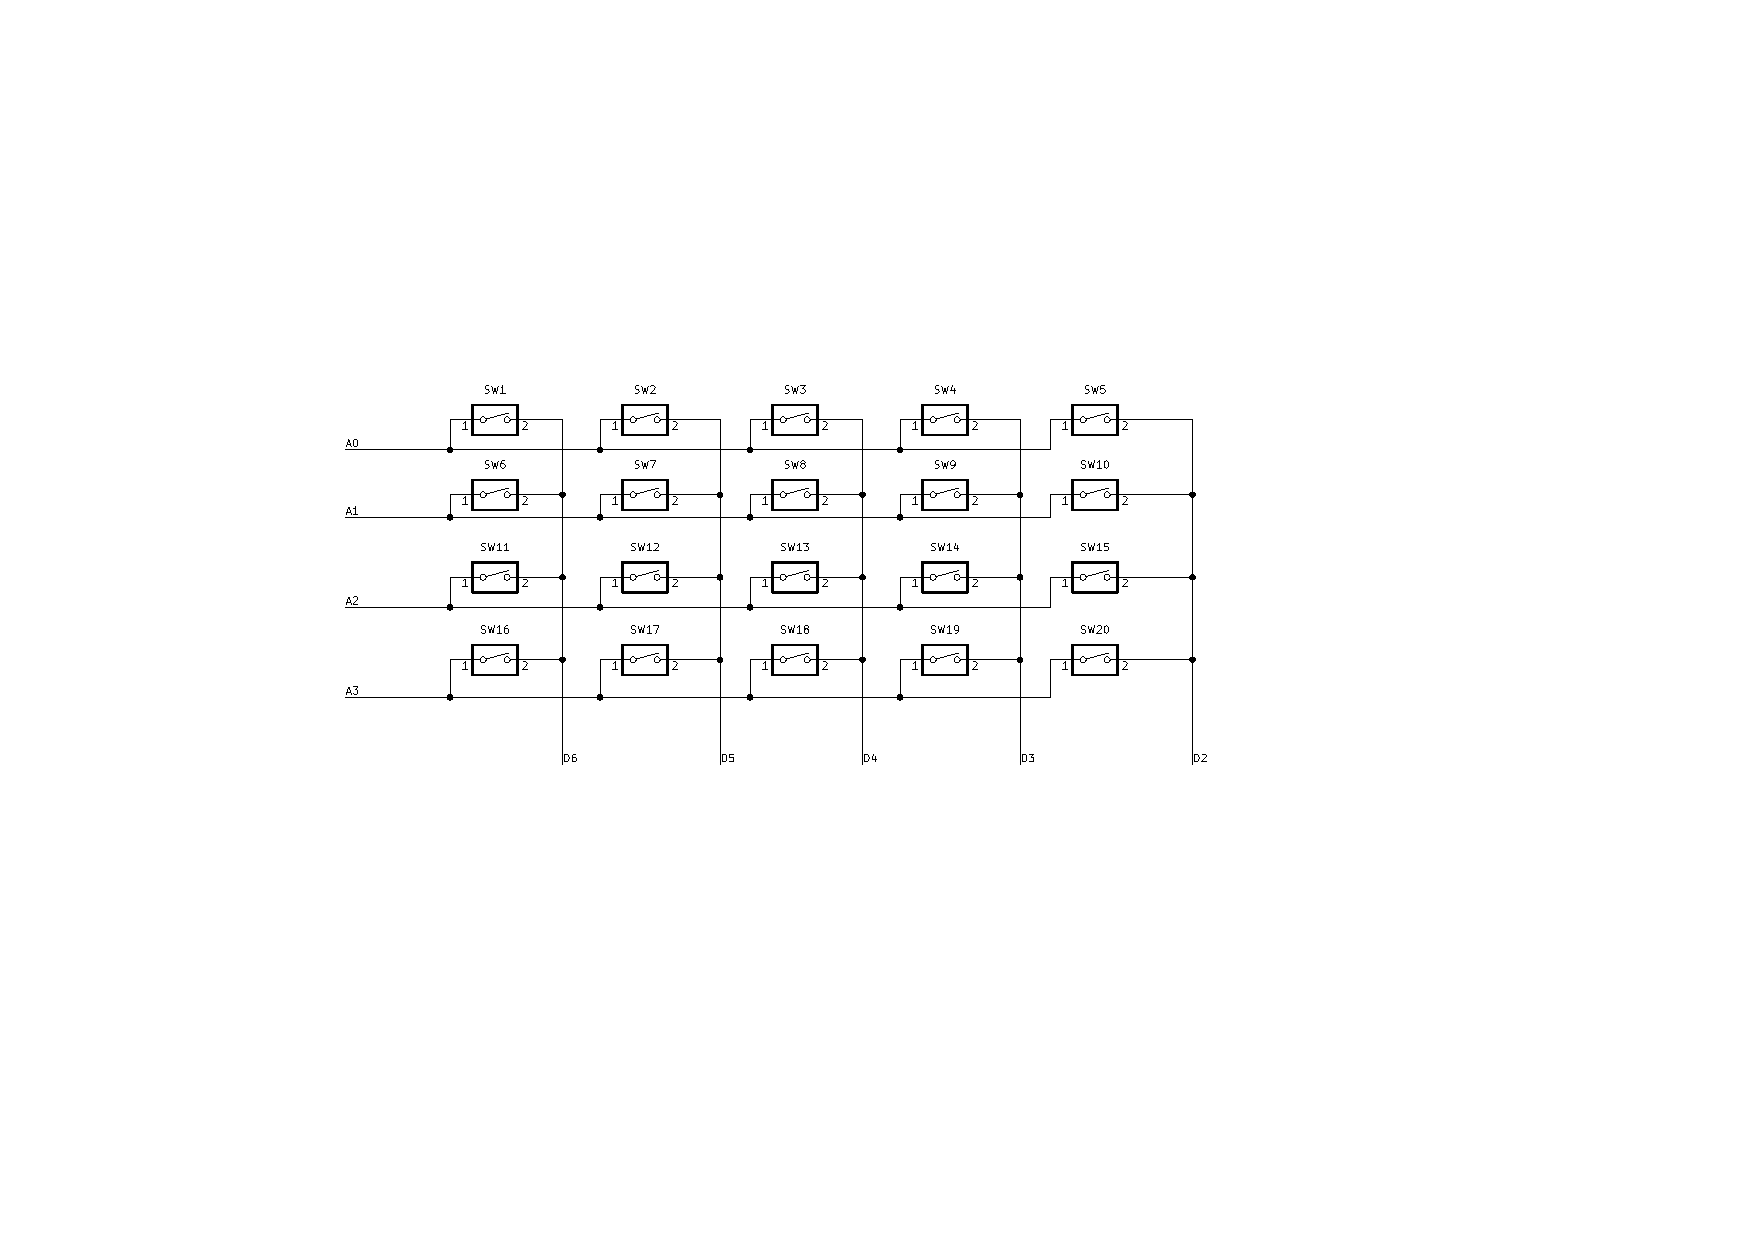
\includegraphics[scale=1]{keypad}
	\end{center}	
	\caption{Схема матричной клавиатуры}
	\end{figure}	
	
	Для обработки клавиш потребовалась библиотека. В Arduino IDE для этих целей есть <<Keypad.h>> \cite{keypad}. Эта библиотека предназначена для работы с матричными клавиатурами. Она позволяет считывать нажатия клавиш и определять, какая именно клавиша была нажата. После её подключения нужно определить объект класса Keypad и задать параметры его работы, такие как количество строк и столбцов, которые есть в клавиатуре. В нашем случае клавиатура 4х5. Необходимости использовать внешние резисторы или диоды нет, так как библиотека использует внутренние подтягивающие резисторы в микроконтроллере и дополнительно обеспечивает высокое входное сопротивление на всех неиспользуемых выводах столбцов.
	
	В листинге 2.2 мы определяем, что наша клавиатура содержит 4 строки и 5 столбцов, а также задаем, какие символы соответствуют каким клавишам. Затем мы указываем, к каким пинам на Arduino подключены строки и столбцы клавиатуры. После этого, используя метод customKeypad.getKey() считываем нажатие клавиш. 
	
	\begin{code}
	\captionof{listing}{Инициализация матричной клавиатуры}
	\begin{minted}
	[
	frame=lines,
	framesep=2mm,
	baselinestretch=1.2,
	%fontsize=\footnotesize,
	linenos,
	breaklines
	]
	{cpp}
#include <Keypad.h>
const byte ROWS = 4;
const byte COLS = 5;
char button;
char keys[ROWS][COLS] = {  // раскладка клавиатуры
  { '0', '1', '2', '3', 'h' },
  { '4', '5', '6', '7', 'x' },
  { '8', '9', 'A', 'B', 's' },
  { 'C', 'D', 'E', 'F', 'd' }
};
byte rowPins[ROWS] = { A0, A1, A2, A3 };  // подключение к строкам клавиатуры
byte colPins[COLS] = { 6, 5, 4, 3, 2 };   // подключение к столбцам клавиатуры
Keypad customKeypad = Keypad(makeKeymap(keys), rowPins, colPins, ROWS, COLS); // инициализация клавиатуры

void loop() {
  button = customKeypad.getKey();  // определение нажатой кнопки
}
	\end{minted}
	\end{code}
	
	
	Для обработки кнопок была написана функция detectbuttons (листинг 2.3). На вход подпрограммы ничего не поступает и никаких значений она не возвращает. Функция вызывает нужную подпрограмму по нажатой клавише. Рисунок 2.2 поясняет ход работы подпрограммы. 
	
	\begin{code}
	\captionof{listing}{Функция обработки кнопок}
	\begin{minted}
	[
	frame=lines,
	framesep=2mm,
	baselinestretch=1.2,
	%fontsize=\footnotesize,
	linenos,
	breaklines
	]
	{cpp}
void detectbuttons() {
  switch (button) {
    case '0':
      //    Serial.println("Button 0");
      append_cmd(0x0000);
      break;

    ...
    
    case 'F':
      //    Serial.println("Button F");
      append_cmd(0x000F);
      break;

    case 's':
      //    Serial.println("Button send");
      pack[0] = cmd;
      pack[1] = cmd >> 8;
      digitalWrite(SS, LOW);
      for (int i = 0; i < 2; i++)
        SPI.transfer(pack[i]);
      digitalWrite(SS, HIGH);
      delay(1000);
      break;

    case 'd':
      //    Serial.println("Button del");
      cmd = cmd >> 4;
      break;

    case 'h':  //help
      do {
        myOLED.clrScr();
        myOLED.print("Help", CENTER, 0);
        myOLED.print("0 1 2 3 h", CENTER, 16);
        myOLED.print("4 5 6 7 x", CENTER, 26);
        myOLED.print("8 9 A B s", CENTER, 36);
        myOLED.print("C D E F d", CENTER, 46);
        myOLED.update();
        button = customKeypad.getKey();
        detectbuttons();
      } while (!button);
      cmd = 0x0000;
      break;
  }
}
	\end{minted}
	\end{code}
	
	\begin{figure}[H]
	\begin{center}
	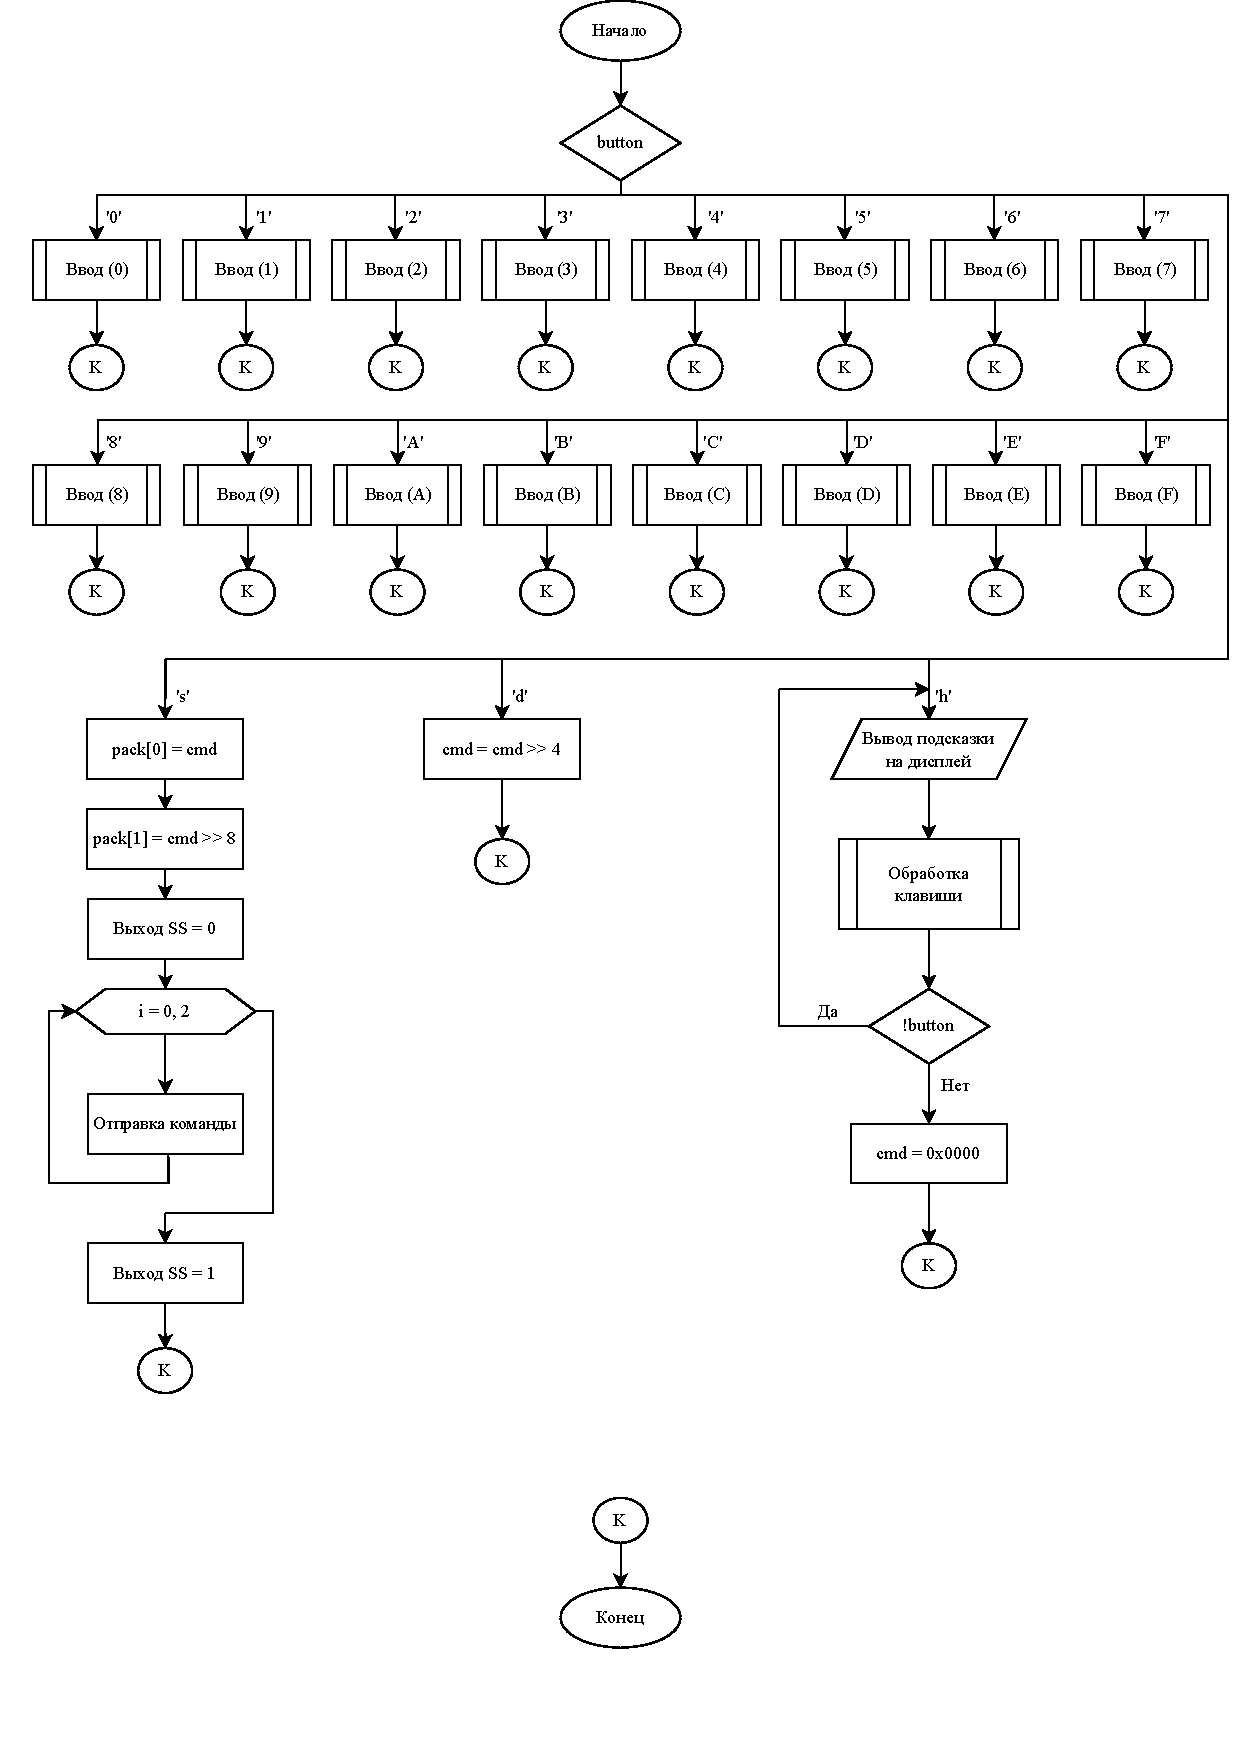
\includegraphics[scale=0.8]{detectbuttons}
	\end{center}	
	\caption{Блок-схема подпрограммы обработки кнопок.}
	\end{figure}	
	
	Для ввода команды была написана функция append\_cmd (листинг 2.4). Подпрограмма  только принимает. На вход поступает, вводимый пользователем набор бит, а далее записывается в команду. Ход работы поясняется на рисунке 2.3. 
	\begin{code}
	\captionof{listing}{Функция ввода команды}
	\begin{minted}
	[
	frame=lines,
	framesep=2mm,
	baselinestretch=1.2,
	%fontsize=\footnotesize,
	linenos,
	breaklines
	]
	{cpp}
void append_cmd(uint16_t comand) {
  if (cmd == 0) {
    cmd = comand;
  } else {
    cmd = cmd << 4;
    cmd |= comand;
  }
}
	\end{minted}
	\end{code}
	
	\begin{figure}[H]
	\begin{center}
	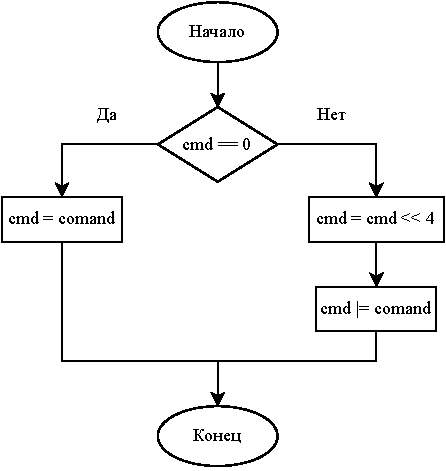
\includegraphics[scale=1]{append_cmd}
	\end{center}	
	\caption{Блок-схема подпрограммы ввода команды.}
	\end{figure}	
	
	В качестве устройства вывода был выбран OLED дисплей. У данного индикатора пиксели излучают свет сами, изображение получается более контрастным и насыщенным, с хорошим углом обзора. Ко всему этому у индикатора низкое энергопотребление. Имеет разрешение 128 на 64 точек, управляется по интерфейсу I2C, графический чип SSD1306 и питается от 3 --- 5 В. Для работы с ним была выбрана библиотека <<OLED\_I2C.h>> за её простоту и лёгкость \cite{oled}. Сам же дисплей нужен для отображения команды, которую вводит пользователь.
	
	\begin{code}
	\captionof{listing}{Вывод команды на дисплей}
	\begin{minted}
	[
	frame=lines,
	framesep=2mm,
	baselinestretch=1.2,
	%fontsize=\footnotesize,
	linenos,
	breaklines
	]
	{cpp}
#include <OLED_I2C.h>
OLED myOLED(SDA, SCL);
extern uint8_t SmallFont[];
uint16_t cmd;
void setup() {
myOLED.begin();
myOLED.setFont(SmallFont);
myOLED.clrScr();
myOLED.update();
}

void loop() {
myOLED.clrScr();
myOLED.print(String(cmd, HEX), CENTER, 25);  //выводим на экран вводимую команду
myOLED.update();
}
	\end{minted}
	\end{code}
	
	Полный код программы приведён в приложении. После успешной компиляции среда разработки вывело сообщение о том, что программа использует 6892 байт (21\%) памяти устройства. Всего доступно 32256 байт. 
	\newpage
	Блок-схема на рисунке 2.4 поясняет работу программы.
	\begin{figure}[H]
	\begin{center}
	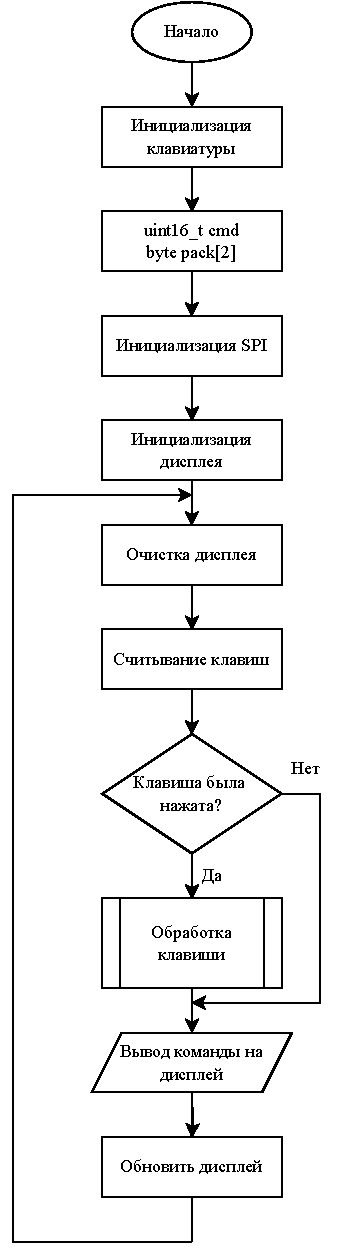
\includegraphics[scale=1]{main}
	\end{center}	
	\caption{Блок-схема главной программы.}
	\end{figure}	
	
	\newpage
	Макет описывается следующей функциональной схемой (рис. 2.5). Подключение клавиатуры может быть осуществлено к любым свободным пинам. В нашем случае строки подключаются к аналоговым пинам 0, 1, 2, 3, а столбцы к цифровым 6, 5, 4, 3, 2. Дисплей подключен по шине I2C, а линии SPI идут к ведомому устройству. 
	\begin{figure}[H]
	\begin{center}
	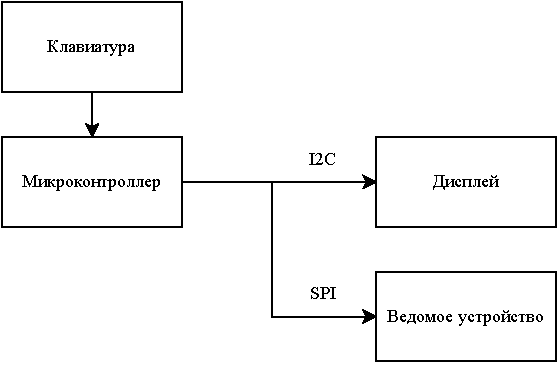
\includegraphics[scale=1]{scheme}
	\end{center}	
	\caption{Функциональная схема SPI тестера.}
	\end{figure}	
	
		
\chapter{Описание работы устройства}
	Процесс работы пользователя с устройством можно представить следующей структурной схемой (рис.3.1). 
	\begin{figure}[H]
	\begin{center}
	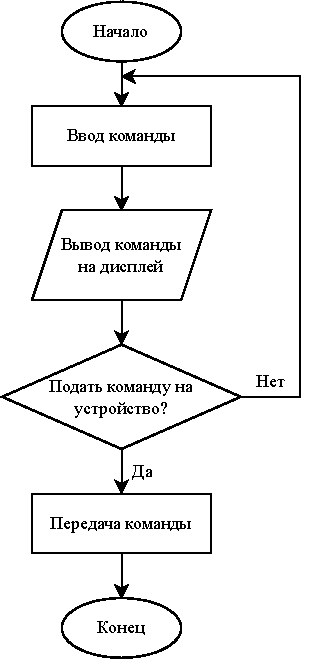
\includegraphics[scale=1]{struct} 
	\end{center}	
	\caption{Структурная схема работы устройства.}
	\end{figure}	
	
	Как упоминалось ранее устройством ввода является матричная клавиатура. Кроме клавиш для ввода команды на ней расположены клавиши вызова подсказки с раскладкой клавиатуры <<h>>, обратный пробел <<d>> и кнопка отправки команды <<s>>. Клавиша <<x>> не назначена и может в будущем быть использована. Всё рабочее время устройство ожидает ввода команды и выводит текущее значение на дисплей. Когда пользователь ввёл команду и хочет её отправить он нажимает кнопку <<s>>. После чего формируется посылка из двух пакетов по одному байту, линия выбора ведомого переходит в низкий уровень и начинается отправка команды. По окончанию отправки линия переходит обратно в высокий уровень. 

	В качестве ведомого устройства для тестов был выбран портативный четырехканальный логический анализатор Miniware MiniDSO LA104. На рисунке 3.2 изображены результаты отправки команд с тестера.
	
\begin{figure}[H]
\centering
\begin{subfigure}[t]{0.45\textwidth}
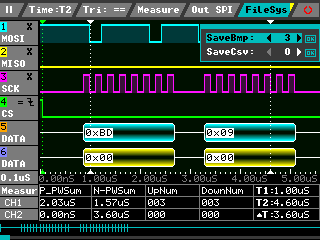
\includegraphics[width=1\textwidth]{test1}
\caption{0x09BD}
\end{subfigure}
\hfill     
\begin{subfigure}[t]{0.45\textwidth}
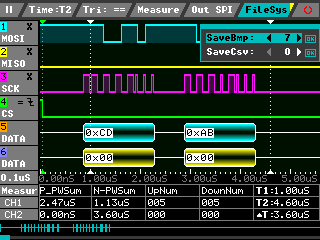
\includegraphics[width=1\textwidth]{test2}
\caption{0xABCD}
\end{subfigure}
\hfill         
\begin{subfigure}[t]{0.45\textwidth}
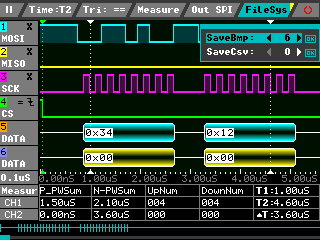
\includegraphics[width=1\textwidth]{test3}
\caption{0x1234}
\end{subfigure}
\hfill         
\begin{subfigure}[t]{0.45\textwidth}
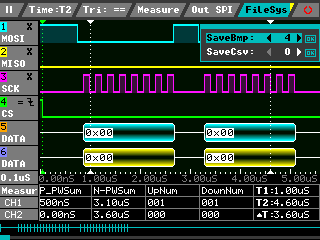
\includegraphics[width=1\textwidth]{test4}
\caption{0x0000}
\end{subfigure}     
\caption{Данные с анализатора.}
\end{figure}

	\newpage
	Проверим нашу заявленную частоту синхронизации 4 МГц (рис. 3.3). 
    \begin{figure}[H]
	\begin{center}
	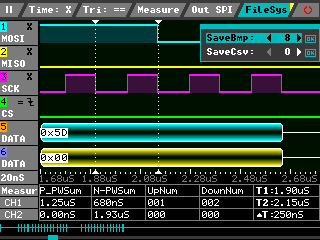
\includegraphics[scale=1]{testfreq} 
	\end{center}	
	\caption{Измерение частоты тактового сигнала.}
	\end{figure}	
	
	Установим флаги $T1$ и $T2$ на начало и конец периода синхросигнала и узнаем его длину, а затем вычислим частоту. 
	
	$\Delta T=T2-T1=250$ нс.
	
	$f=\dfrac{1}{\Delta T}=\dfrac{1}{250 \cdot 10^{-9}}=4$ МГц.
	
	Таким образом, макет тестера ведомых SPI устройств является работоспособным. Частота и отсылаемые команды были подтверждены с помощью логического анализатора.
	

\chapter*{Заключение}
\addcontentsline{toc}{chapter}{Заключение} 
	В результате научно-исследовательской работы были выполнены следующие задачи:
	\begin{enumerate}
		\item Выбраны инструменты для разработки программы.
		\item Разработана программа.
		\item Собран макет.
		\item Проверена работоспособность.
	\end{enumerate}
	
	По итогам работы цель достигнута: создан рабочий макет тестера ведомых SPI устройств. 
\newpage
\addcontentsline{toc}{chapter}{Список использованной литературы}
\printbibliography[title={Список использованной литературы}] 

\newpage
\chapter*{\raggedleft\label{appendix1}Приложение}
\section*{Текст программы}
\begin{code}
\captionof*{listing}{Тестер ведомых SPI устройств}
	\begin{minted}
	[
	frame=lines,
	framesep=2mm,
	baselinestretch=1.2,
	%fontsize=\footnotesize,
	linenos,
	breaklines
	]
	{cpp}
#include <SPI.h>
#include <OLED_I2C.h>
OLED myOLED(SDA, SCL);
extern uint8_t SmallFont[];
#include <Keypad.h>
const byte ROWS = 4;
const byte COLS = 5;
char button;
char keys[ROWS][COLS] = {
  { '0', '1', '2', '3', 'h' },
  { '4', '5', '6', '7', 'x' },
  { '8', '9', 'A', 'B', 's' },
  { 'C', 'D', 'E', 'F', 'd' }
};
byte rowPins[ROWS] = { A0, A1, A2, A3 };  // подключение к строкам клавиатуры
byte colPins[COLS] = { 6, 5, 4, 3, 2 };   // подключение к столбцам клавиатуры
Keypad customKeypad = Keypad(makeKeymap(keys), rowPins, colPins, ROWS, COLS);
uint16_t cmd;
byte pack[2];
void setup() {
  //Serial.begin(9600);
  SPI.begin();
  myOLED.begin();
  myOLED.setFont(SmallFont);
  myOLED.clrScr();
  myOLED.update();
}

void loop() {
  myOLED.clrScr();
  button = customKeypad.getKey();  // определение нажатой кнопки
  if (button != NO_KEY)
    detectbuttons();
  //Serial.println(button);
  myOLED.print(String(cmd, HEX), CENTER, 25);  //выводим на экран вводимую команду
  myOLED.update();
}


void append_cmd(uint16_t comand) {
  if (cmd == 0) {
    cmd = comand;
  } else {
    cmd = cmd << 4;
    cmd |= comand;
  }
}

void detectbuttons() {
  switch (button) {
    case '0':
      //    Serial.println("Button 0");
      append_cmd(0x0000);
      break;

    case '1':
      //    Serial.println("Button 1");
      append_cmd(0x0001);
      break;

    case '2':
      //    Serial.println("Button 2");
      append_cmd(0x0002);
      break;

    case '3':
      //    Serial.println("Button 3");
      append_cmd(0x0003);
      break;

    case '4':
      //    Serial.println("Button 4");
      append_cmd(0x0004);
      break;

    case '5':
      //    Serial.println("Button 5");
      append_cmd(0x0005);
      break;

    case '6':
      //    Serial.println("Button 6");
      append_cmd(0x0006);
      break;

    case '7':
      //    Serial.println("Button 7");
      append_cmd(0x0007);
      break;

    case '8':
      //    Serial.println("Button 8");
      append_cmd(0x0008);
      break;

    case '9':
      //    Serial.println("Button 9");
      append_cmd(0x0009);
      break;

    case 'A':
      //    Serial.println("Button A");
      append_cmd(0x000A);
      break;

    case 'B':
      //    Serial.println("Button B");
      append_cmd(0x000B);
      break;

    case 'C':
      //    Serial.println("Button C");
      append_cmd(0x000C);
      break;

    case 'D':
      //    Serial.println("Button D");
      append_cmd(0x000D);
      break;

    case 'E':
      //    Serial.println("Button E");
      append_cmd(0x000E);
      break;

    case 'F':
      //    Serial.println("Button F");
      append_cmd(0x000F);
      break;

    case 's':
      //    Serial.println("Button send");
      pack[0] = cmd;
      pack[1] = cmd >> 8;
      digitalWrite(SS, LOW);
      for (int i = 0; i < 2; i++)
        SPI.transfer(pack[i]);
      digitalWrite(SS, HIGH);
      break;

    case 'd':
      //    Serial.println("Button del");
      cmd = cmd >> 4;
      break;

    case 'h':  //help
      do {
        myOLED.clrScr();
        myOLED.print("Help", CENTER, 0);
        myOLED.print("0 1 2 3 h", CENTER, 16);
        myOLED.print("4 5 6 7 x", CENTER, 26);
        myOLED.print("8 9 A B s", CENTER, 36);
        myOLED.print("C D E F d", CENTER, 46);
        myOLED.update();
        button = customKeypad.getKey();
        detectbuttons();
      } while (!button);
      cmd = 0x0000;
      break;
  }
}

	\end{minted}
	\end{code}
\end{document}

